\subsubsection{First-order scheme}
\label{subsec:revised-numerical-first}
\Cref{tab:first-order-errors} gives the errors and observed orders;
\Cref{fig:first-order-convergence-rates} shows the corresponding
log--log error curves. On the finest refinement interval, the rates
for $\bs u,\bs\omega,\bs m,\bs k,\varphi,\bs H$ are
1.019, 0.994, 0.999, 0.997, 1.018, and 1.017, respectively.
The modified pressure exhibits a rate of 2.065 in this test.
The sampled curl diagnostic remains between $1.22\times10^{-13}$
and $8.51\times10^{-12}$, consistent with the discrete gradient
recovery of the magnetic field up to numerical error.

\begin{table}[htbp]
\centering
\caption{Relative errors and observed rates for the first-order scheme, $T=2$ and $\dt=1/K$. $C_H$ is the sampled absolute curl diagnostic.}
\label{tab:first-order-errors}
\begingroup
\small
\setlength{\tabcolsep}{3.5pt}
\renewcommand{\arraystretch}{1.15}
\begin{tabular}{crrrrrrrr}
\toprule
\multicolumn{9}{c}{(a) Velocity, pressure, angular velocity, and magnetization}\\
\midrule
$K$ & \multicolumn{2}{c}{$\bs u$: $H^1$} & \multicolumn{2}{c}{$\widetilde p$: $L^2$} & \multicolumn{2}{c}{$\bs\omega$: $H^1$} & \multicolumn{2}{c}{$\bs m$: $H(\div)$}\\
 & Error & Rate & Error & Rate & Error & Rate & Error & Rate\\
\midrule
4 & $9.6554\!\times\!10^{-1}$ & -- & $5.6019\!\times\!10^{-1}$ & -- & $6.4182\!\times\!10^{-1}$ & -- & $3.9160\!\times\!10^{-1}$ & --\\
8 & $4.3070\!\times\!10^{-1}$ & 1.165 & $1.0260\!\times\!10^{-1}$ & 2.449 & $3.5671\!\times\!10^{-1}$ & 0.847 & $1.9873\!\times\!10^{-1}$ & 0.979\\
16 & $1.9858\!\times\!10^{-1}$ & 1.117 & $2.1172\!\times\!10^{-2}$ & 2.277 & $1.8331\!\times\!10^{-1}$ & 0.960 & $9.9738\!\times\!10^{-2}$ & 0.995\\
32 & $9.8002\!\times\!10^{-2}$ & 1.019 & $5.0596\!\times\!10^{-3}$ & 2.065 & $9.2018\!\times\!10^{-2}$ & 0.994 & $4.9919\!\times\!10^{-2}$ & 0.999\\
\bottomrule
\end{tabular}
\par\medskip
\begin{tabular}{crrrrrrr}
\toprule
\multicolumn{8}{c}{(b) Auxiliary curl field, potential, magnetic field, and curl diagnostic}\\
\midrule
$K$ & \multicolumn{2}{c}{$\bs k$: $L^2$} & \multicolumn{2}{c}{$\varphi$: $H^1$} & \multicolumn{2}{c}{$\bs H$: $H(\curl)$} & $C_H$\\
 & Error & Rate & Error & Rate & Error & Rate &\\
\midrule
4 & $5.1511\!\times\!10^{-1}$ & -- & $6.5848\!\times\!10^{-1}$ & -- & $6.6223\!\times\!10^{-1}$ & -- & $1.2220\!\times\!10^{-13}$\\
8 & $2.6813\!\times\!10^{-1}$ & 0.942 & $3.7678\!\times\!10^{-1}$ & 0.805 & $3.7965\!\times\!10^{-1}$ & 0.803 & $5.1946\!\times\!10^{-13}$\\
16 & $1.3523\!\times\!10^{-1}$ & 0.988 & $1.8757\!\times\!10^{-1}$ & 1.006 & $1.8935\!\times\!10^{-1}$ & 1.004 & $2.0267\!\times\!10^{-12}$\\
32 & $6.7750\!\times\!10^{-2}$ & 0.997 & $9.2620\!\times\!10^{-2}$ & 1.018 & $9.3572\!\times\!10^{-2}$ & 1.017 & $8.5067\!\times\!10^{-12}$\\
\bottomrule
\end{tabular}
\endgroup
\end{table}

\begin{figure}[htbp]
\centering
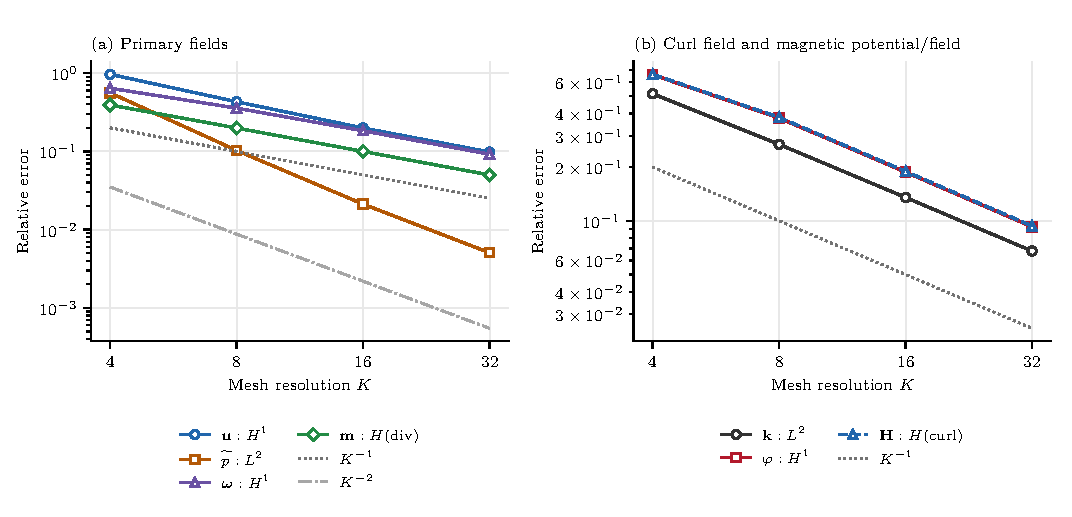
\includegraphics[width=\textwidth]{figures/first_order_errors.pdf}
\caption{Relative errors for the first-order discretization under joint
refinement with $\dt=1/K$.
(a) Velocity, modified pressure, angular velocity, and magnetization.
(b) Auxiliary curl field, magnetic potential, and magnetic field.
The horizontal coordinate is the mesh resolution $K=4,8,16,32$, so
refinement proceeds from left to right. Reference lines proportional
to $K^{-1}$ and $K^{-2}$ indicate first- and second-order decay with
mesh refinement, not independently measured temporal orders.}
\label{fig:first-order-convergence-rates}
\end{figure}

\FloatBarrier
